\documentclass[17pt]{beamer} %Makes presentation
%\documentclass[handout]{beamer} %Makes Handouts
\usetheme{Singapore} %Gray with fade at top
\useoutertheme[subsection=false]{miniframes} %Supppress subsection in header
\useinnertheme{rectangles} %Itemize/Enumerate boxes
\usecolortheme{seagull} %Color theme
\usecolortheme{rose} %Inner color theme

\definecolor{light-gray}{gray}{0.75}
\definecolor{dark-gray}{gray}{0.55}
\setbeamercolor{item}{fg=light-gray}
\setbeamercolor{enumerate item}{fg=dark-gray}

\setbeamertemplate{navigation symbols}{}
%\setbeamertemplate{mini frames}[default]
%\setbeamercovered{dynamics}
\setbeamerfont*{title}{size=\Large,series=\bfseries}
\setbeamerfont{footnote}{size=\tiny}

%\setbeameroption{notes on second screen} %Dual-Screen Notes
%\setbeameroption{show only notes} %Notes Output

\setbeamertemplate{frametitle}{\vspace{.5em}\bfseries\insertframetitle}
\newcommand{\heading}[1]{\noindent \textbf{#1}\\ \vspace{1em}}

\usepackage{bbding,color,multirow,times,ccaption,tabularx,graphicx,verbatim,booktabs}
\usepackage{colortbl} %Table overlays
\usepackage[english]{babel}
%\usepackage[latin1]{inputenc}
%\usepackage[T1]{fontenc}
\usepackage{lmodern}

%\author[]{Thomas J. Leeper}
\institute[]{
  \inst{}%
  Department of Government\\London School of Economics and Political Science
}

\usepackage{tikz}
\usetikzlibrary{shapes,arrows}

\title{Deriving Hypotheses from Theory}

% Hypotheses are the observable implications of theories. How do we derive hypotheses from theories? How do we overcome ``observational equivalence'' wherein multiple theories yield similar expectations about the world? What does it mean to test a hypothesis?


\date[]{}

\begin{document}

\frame{\titlepage}

\frame{\tableofcontents}


\section[News]{Causal Claims in the News}
%\frame{\tableofcontents[currentsection]}


\frame{

\frametitle{Causal Claims in the News}

\begin{itemize}\itemsep0.5em
\item Share news stories
\item What was the claim?
\item Was there any evidence or test?
\end{itemize}

}

\section{Review of Last Week}
\frame{\tableofcontents[currentsection]}


\frame{

\frametitle{Last Week}

\begin{itemize}
\item What are theories?
	\begin{itemize}
	\item A tentative conjecture about the causes of some phenomenon of interest
	\item An argument that attempts to explain how concepts are causally related
	\end{itemize}
\item Deduction and Induction
\item Evaluating theories
\end{itemize}

}


\frame{

\frametitle{Generality \& Parsimony}

Think for 90 seconds about each of these principles:

\small 

\begin{itemize}\itemsep1em
\item Generality: Theories that can explain more are preferred over theories that can explain less
\item Parsimony: Simple theories are preferred over complex theories
\end{itemize}

\normalsize

Are these principles defensible?\\ Are they any good?

}



\section{Generating Hypotheses}
\frame{\tableofcontents[currentsection]}


\frame{

\frametitle{Hypotheses}

\begin{itemize}
\item<2-> Definition: a theory-based statement about a relationship that we expect to observe.\footnote{Kellstedt and Whitten (p.4)}

\item<3-> Features
	\begin{itemize}
	\item Derived from theory
	\item Specific
	\item Empirical/observable
	\item About variables, not concepts
	\end{itemize}
\end{itemize}

}

% we cannot test theory; we can only test observable implications of theory
% hypotheses are statements about observable implications
% finding support for a hypothesis is evidence in support of a theory
% finding lack of support for a hypothesis is evidence against a theory



\frame{

\frametitle{How do we generate hypotheses?}

\begin{itemize}
\item Think about \textit{observable implications}
\item What would evidence consistent with this theory be?
\item What would evidence inconsistent with this theory be?
	\begin{itemize}
	\item<2-> This is \textit{falsifiability}
	\end{itemize}
\end{itemize}

}

% falsifiability
	% typically talked about in descriptive terms (all swans are white)
	% can be harder to think of non-falsifiable causal arguments
		% theories without observable implications (homeopathy; remote viewing)
		% ethics are non-falsifiable without a predetermined set of rules governing what is and is not ethical

% Examples from Rosenbaum


\frame{

\frametitle{Example: Broad Street Cholera}

\begin{itemize}\itemsep0.5em
\item 1854 outbreak of cholera in London
	\begin{itemize}
	\item around Broad Street (Soho)
	\item 616 eventual deaths
	\end{itemize}
\item<2-> What causes transmission of cholera?
\item<3-> Dominant theory at time: ``miasma''
\item<4-> Hypotheses:
	\begin{itemize}
	\item Clean up garbage $\rightarrow \downarrow$ cholera
	\item Open windows $\rightarrow \downarrow$ cholera
	\end{itemize}
\end{itemize}

}

% miasmatic theory of disease (``bad air''); dominant since the bubonic plague


\frame{

\frametitle{John Snow's Map}

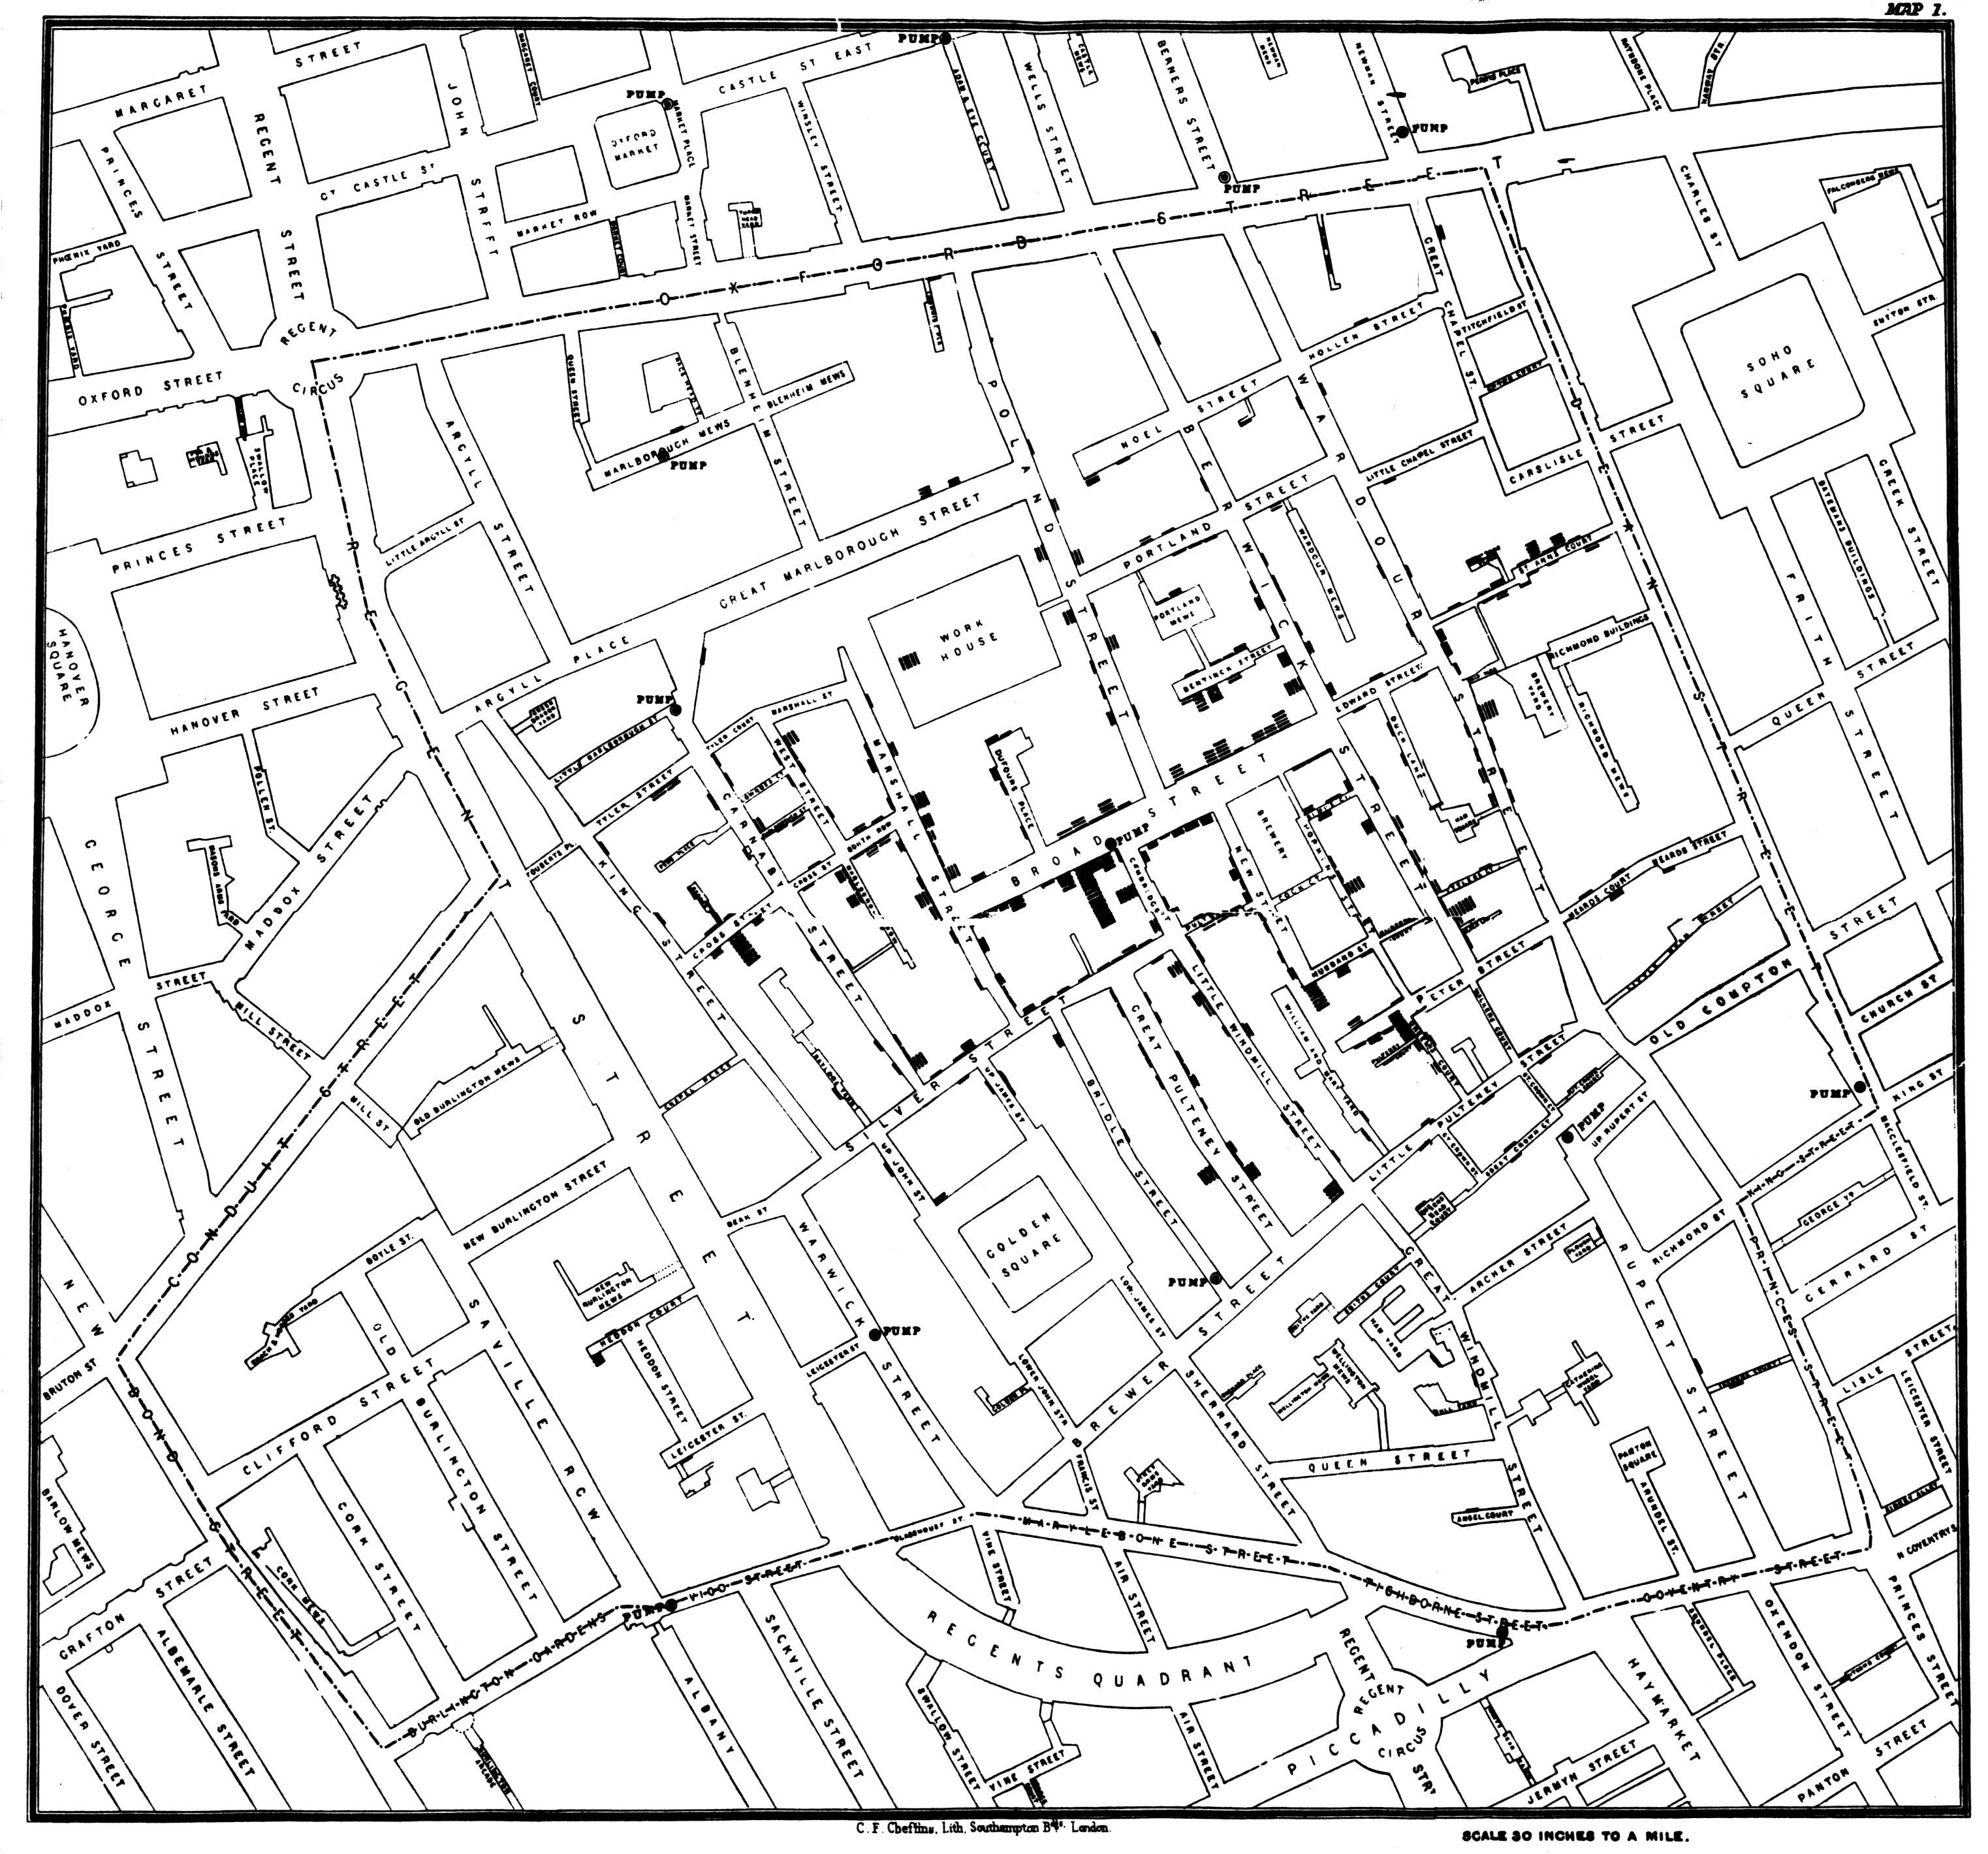
\includegraphics[width=\textwidth]{images/broadstreet}

{\footnotesize Image source: Public Domain from \href{https://en.wikipedia.org/wiki/File:Snow-cholera-map-1.jpg}{Wikipedia}

}

% inductive process: map outbreak of cholera; identify pattern
% new theory: cholera is spread by contaminated water
% hypothesis: removing access to contaminated water reduces cholera infection
% later used as an example of the ``Germ theory of disease'' (most closely associated with Louis Pasteur)



\frame{

\frametitle{Observational Equivalence}

\begin{itemize}
\item Definition: All hypotheses for two (or more) theories are identical
\item What to do?
	\begin{itemize}
	\item Generate more specific expectations % maybe alternative DVs; more fine grained hypothesis; moderators; etc.
	\item Move outside scope conditions
	\item Settle for lack of explanation
	\end{itemize}
\end{itemize}

}



% activity where two theories predict same result

\section{Hypothesis Testing}
\frame{\tableofcontents[currentsection]}


\frame{

\frametitle{Hypothesis Testing}

\begin{itemize}
\item Multiple schools of thought
\item History is conflictual and murky
\item Two strands of literature
	\begin{itemize}
	\item Philosophy of science
	\item Statistics
	\end{itemize}

\end{itemize}

}

% what does it mean to "test" a hypothesis?

\frame{

\frametitle{Two Forms of Hypothesis Testing}

\begin{columns}[T] % align columns
\begin{column}{.4\textwidth}
\begin{block}{Null hypothesis}
Begin with \textit{null hypothesis} (commonly no relationship)

Your hypothesis expects an alternative state of the world

Associated with Ronald Fisher
\end{block}
\end{column}

\begin{column}{.4\textwidth}
\begin{block}{Alternative hypotheses}
Begin with two alternative hypotheses:\\
One from your theory\\
One from an alternative theory\\

Accept hypothesis consistent with observation

Associated with Jerzy Neyman and Egon Pearson
\end{block}
\end{column}
\end{columns}

{\footnotesize You've probably previously been exposed to some blend of these ideas.}

}

% today we want to discuss principles of hypothesis testing as a way of thinking independent of statistics


% thinking counterfactually
	% can we observe the counterfactual (in another case, in the same case at another time, in a collection of other cases)?
	% if not, can we think about what that counterfactual might look like? (see Fearon's use of ``counterfactual method'')



\frame{

\frametitle{A Good Test}

\begin{itemize}
\item Correct level of analysis
\item Within scope conditions of theory
\item Well-defined concepts
\item Measures of high construct validity, accuracy, and precision
\item Possible to observe any correlation between potential cause and potential effect
\item Consistent with or an improvement upon past methods
\item (Well-powered)
\end{itemize}

}


\frame{

\frametitle{Some Testing Challenges}

\begin{enumerate}
\item Deterministic and probabilistic causality
\item Multiple causation, moderation
\item Equifinality
\item Confirmation or disconfirmation bias
\end{enumerate}

}




% multiple specific forms of testing, which we'll be exposed to over the coming weeks
	% case studies and comparisons
	% process tracing
	% tabular and visual comparisons
	% regression
	% experimentation

% realizing that we will always be inductive and we may go into the field to test a theory and end up instead generating a new theory



% distinguish between training set and test set



\section{Preview}
\frame{\tableofcontents[currentsection]}

\frame{

\frametitle{Preview of Next Week}

\begin{itemize}
\item What is a case?
\item What are case studies?
\item How do we use case studies to test and build theories?
\end{itemize}

}



\appendix
\frame{}

\end{document}
